% Appendix A

\chapter{Figures} % Main appendix title

\label{Figures} % For referencing this appendix elsewhere, use \ref{AppendixA}

%%%%% Introduction %%%%%

\begin{figure}[th]
\centering
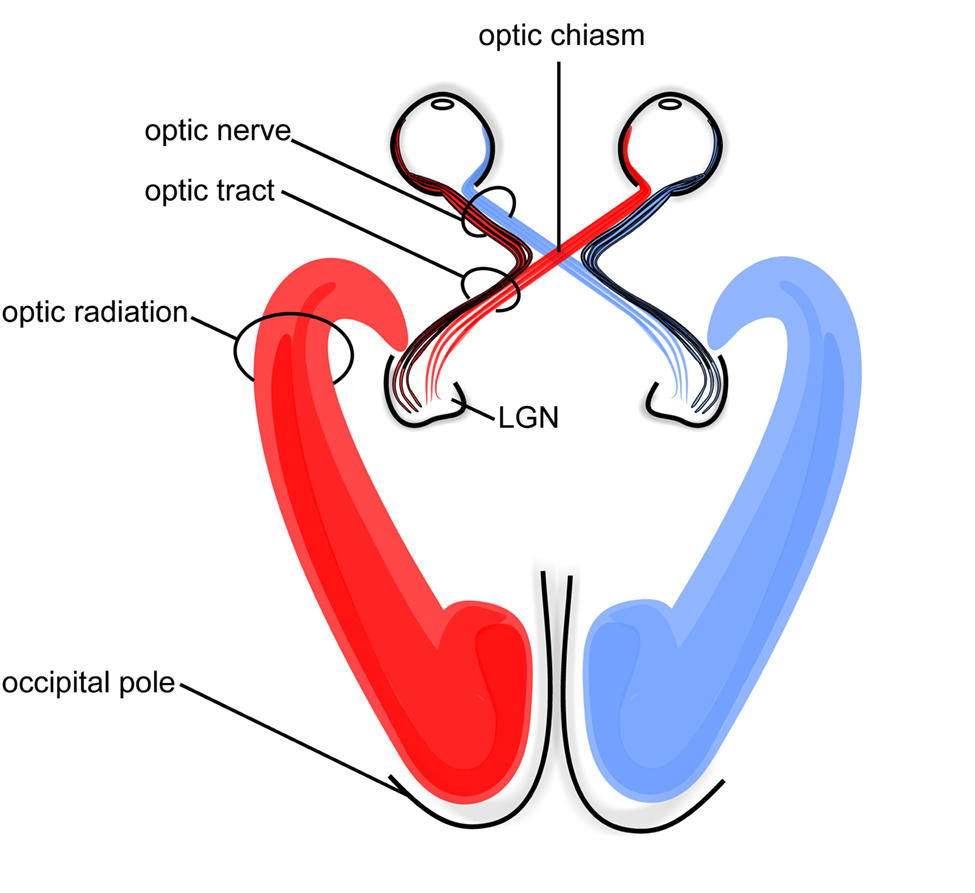
\includegraphics{Figures/visual_system}
\decoRule %puts an aesthetic horizontal line below the image
\caption[Figure]{Schéma des voies visuelles précorticales humaines (adapté de Hofer S. et al., 2010 via Wikimedia Commons [CC BY 3.0])}
\label{fig:visual_system}
\end{figure}

\begin{figure}[th]
\centering
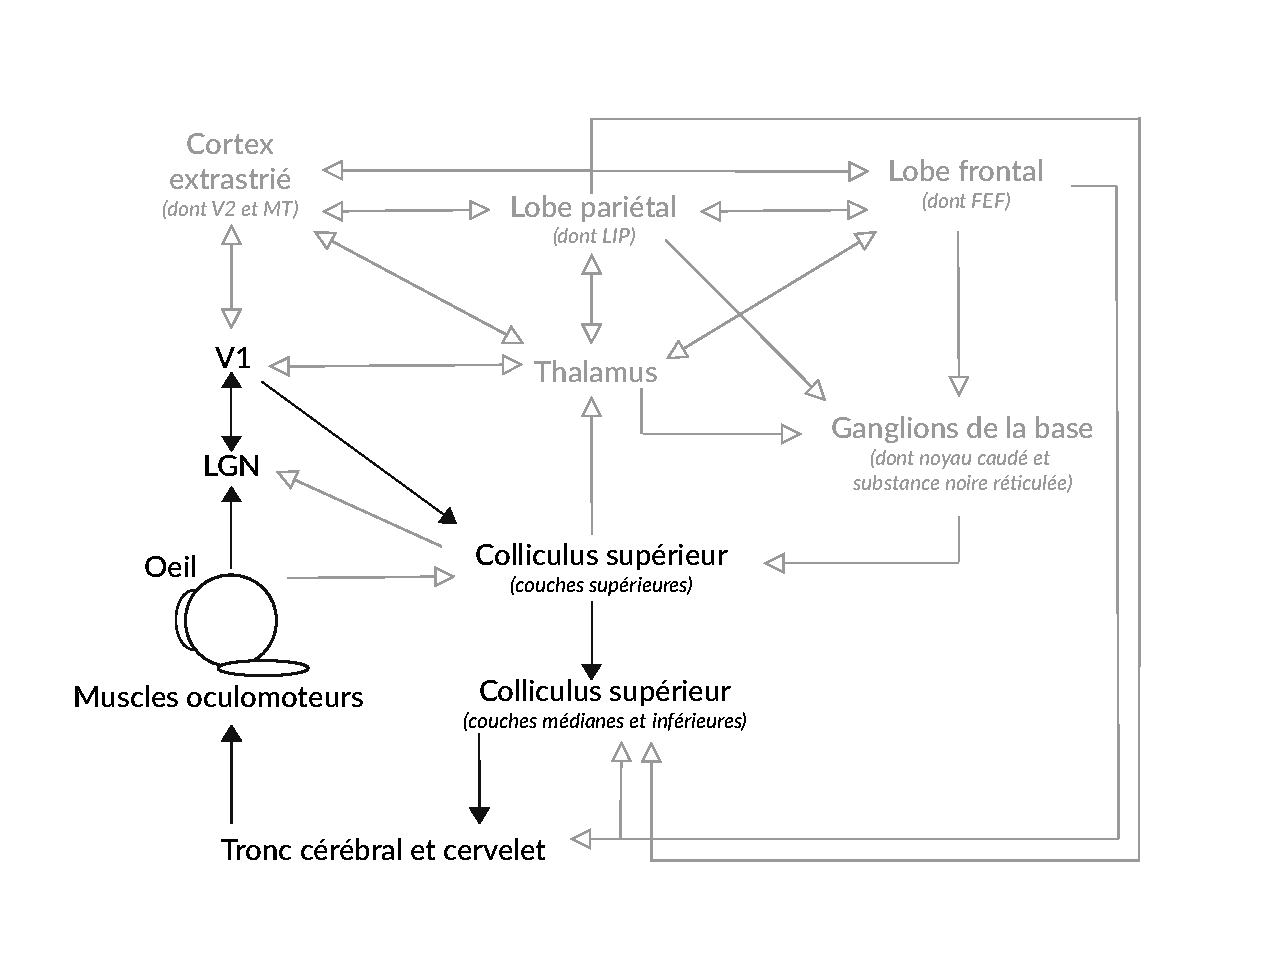
\includegraphics[scale=0.8]{Figures/saccadic_sys}
\decoRule %puts an aesthetic horizontal line below the image
\caption[Figure]{Schéma simplifié du réseau nerveux impliqué dans la planification et l'exécution des saccades oculaires. Les parties noires correspondent aux composantes dont notre modèle tente de modéliser les fonctions, tandis que celles grises correspondent au reste du réseau (adapté de \cite{Zhaoping2014})}
\label{fig:saccadic_sys}
\end{figure}

\begin{figure}[th]
\centering
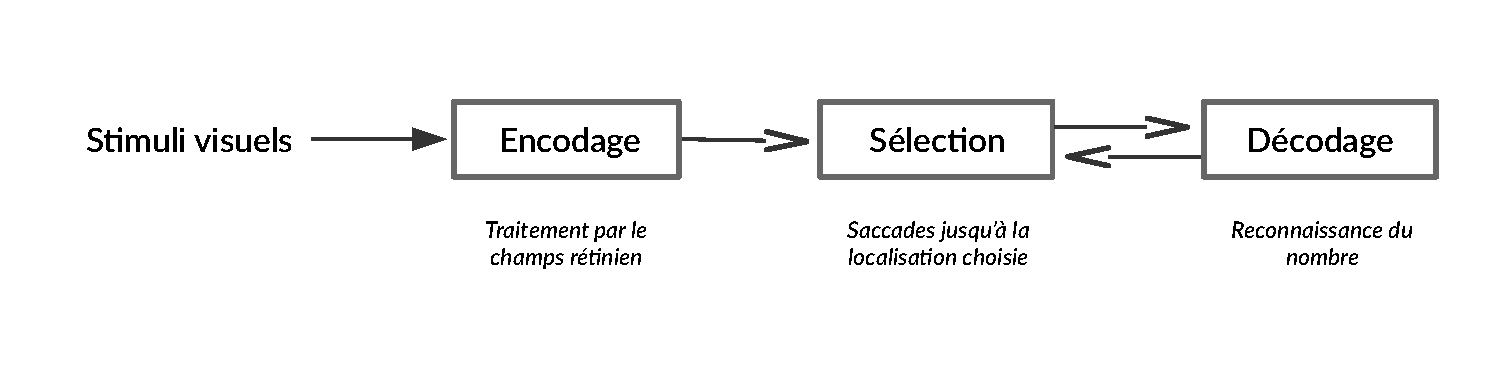
\includegraphics[scale=0.75]{Figures/visual_system_simple}
\decoRule %puts an aesthetic horizontal line below the image
\caption[Figure]{Schéma simplifié du fonctionnement du système visuel avec son \textit{équivalence dans le modèle} (adapté de \cite{Zhaoping2014})}
\label{fig:visual_system_simple}
\end{figure}

%%%%% Matériel et méthodes %%%%%

\begin{table}
\resizebox{19cm}{!}{
\begin{tabular}{| p{4cm} || l | l | p{5cm} | l | l |}
\hline
& Identifiant & Système d'explotation & Processeur & Mémoire vive & Carte graphique\\ \hline
Machine physique & ASUS ROG G75VW & Windows 7 64-bit SP1 & Intel Core I7-3610QM 2,30GHz (8CPU) &  
8 GB (DDR3) & NVIDIA GeForce GTX670M\\ \hline
Machine virtuelle (ressources allouées) & VirtualBox v.5.2.6 & Ubuntu 16.04 & 4 CPU, 90\% des ressources & 
5298 Mo & Support GPU non-utilisé\\ \hline
\end{tabular}
}
\caption[Tableau]{Matériel physique et numérique utilisé pour réaliser les modélisations}
\label{tab:materiel}
\end{table}

\begin{figure}[th]
\centering
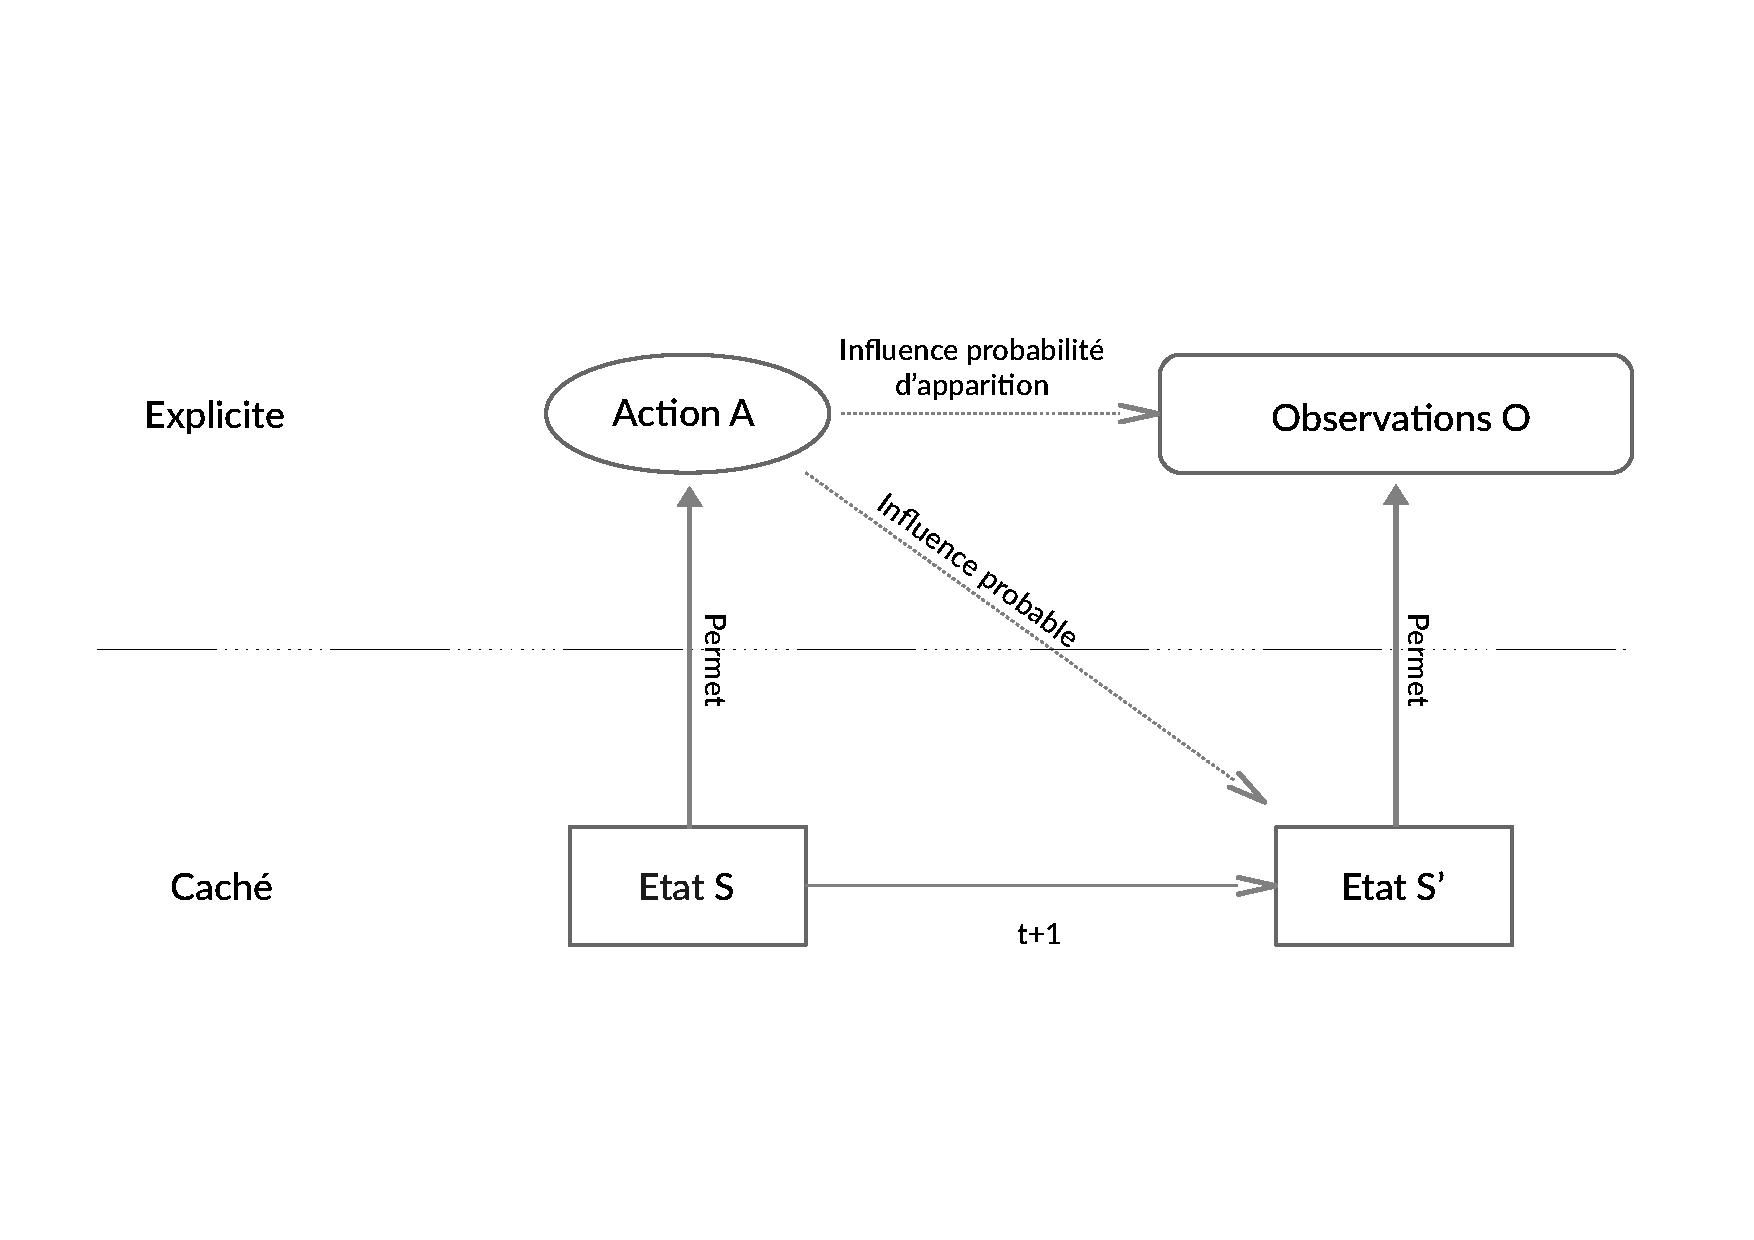
\includegraphics[scale=0.45]{Figures/POMDP}
\decoRule %puts an aesthetic horizontal line below the image
\caption[Figure]{Schéma des interations entre l'agent et son environnement au cours du temps dans un modèle POMDP}
\label{fig:POMDP}
\end{figure}

\begin{figure}[th]
\centering
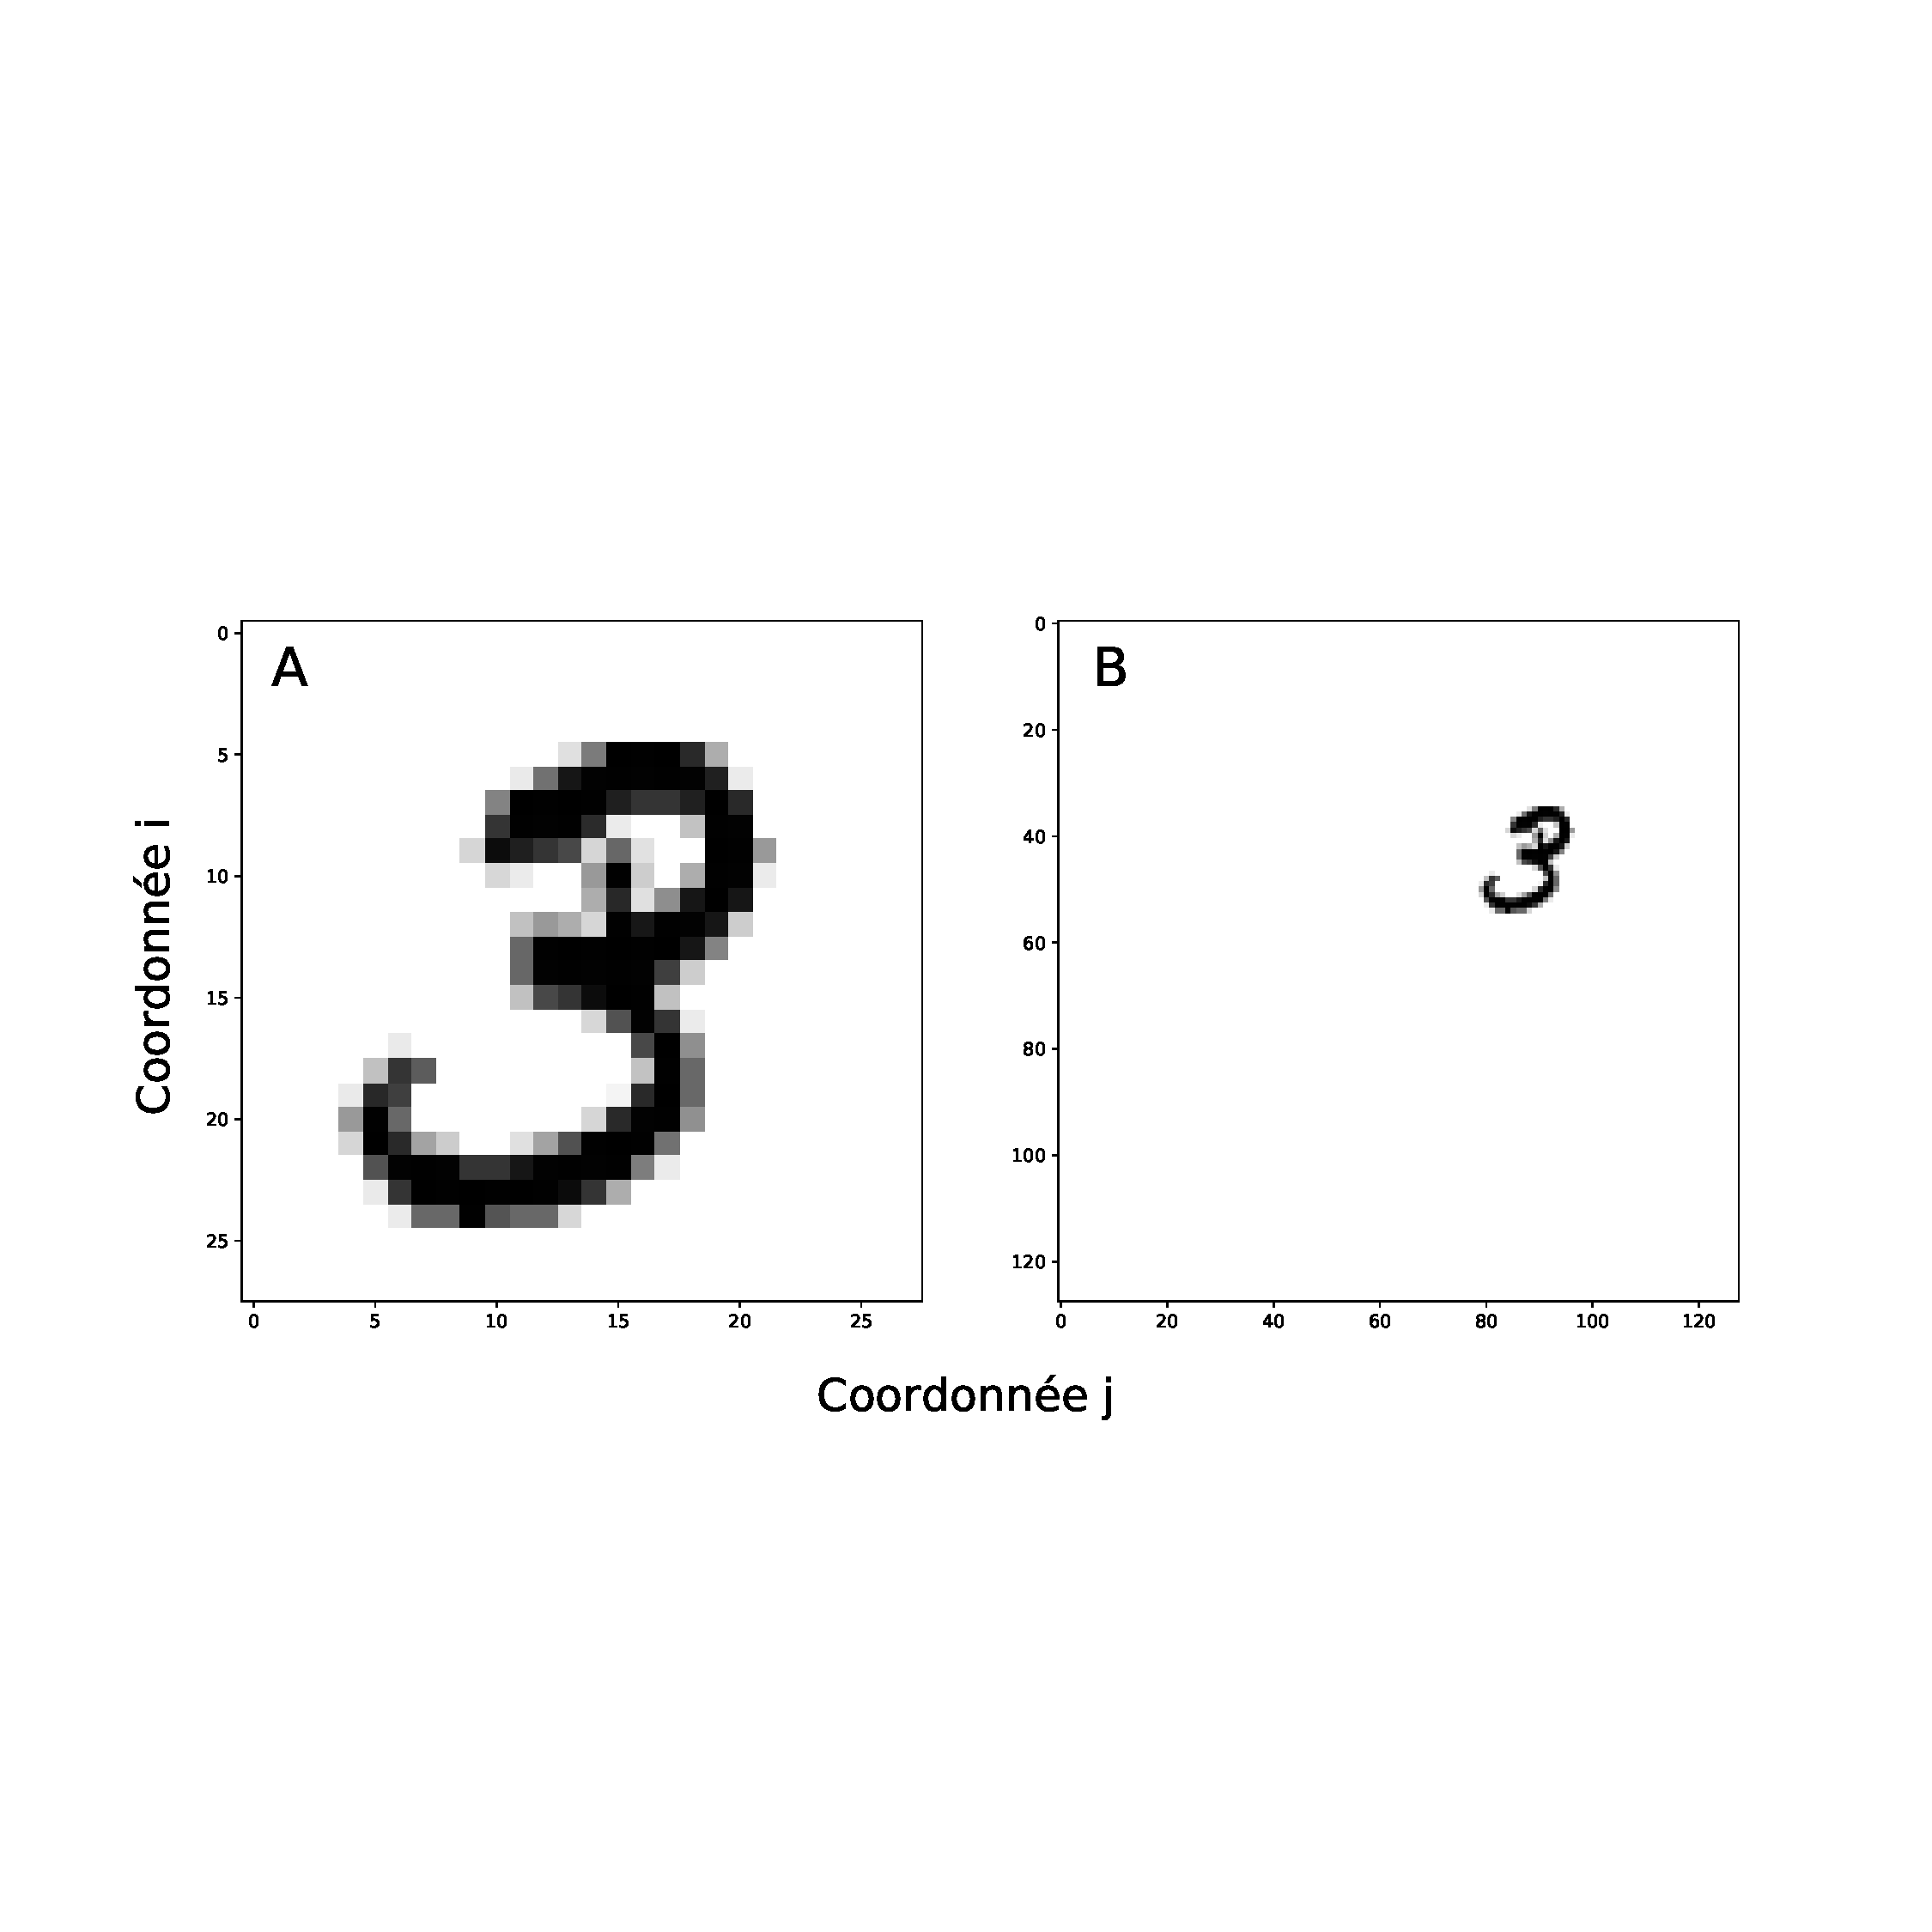
\includegraphics[scale=0.3]{Figures/mnist_reshape}
\decoRule %puts an aesthetic horizontal line below the image
\caption[Figure]{\textbf{A.} Image originale tirée de la base MNIST ; \textbf{B.} Image après translation aux coordonnées $(i=-20,j=25)$ sur un fond blanc $128\times128$}
\label{fig:mnist_reshape}
\end{figure}

\begin{figure}[th]
\centering
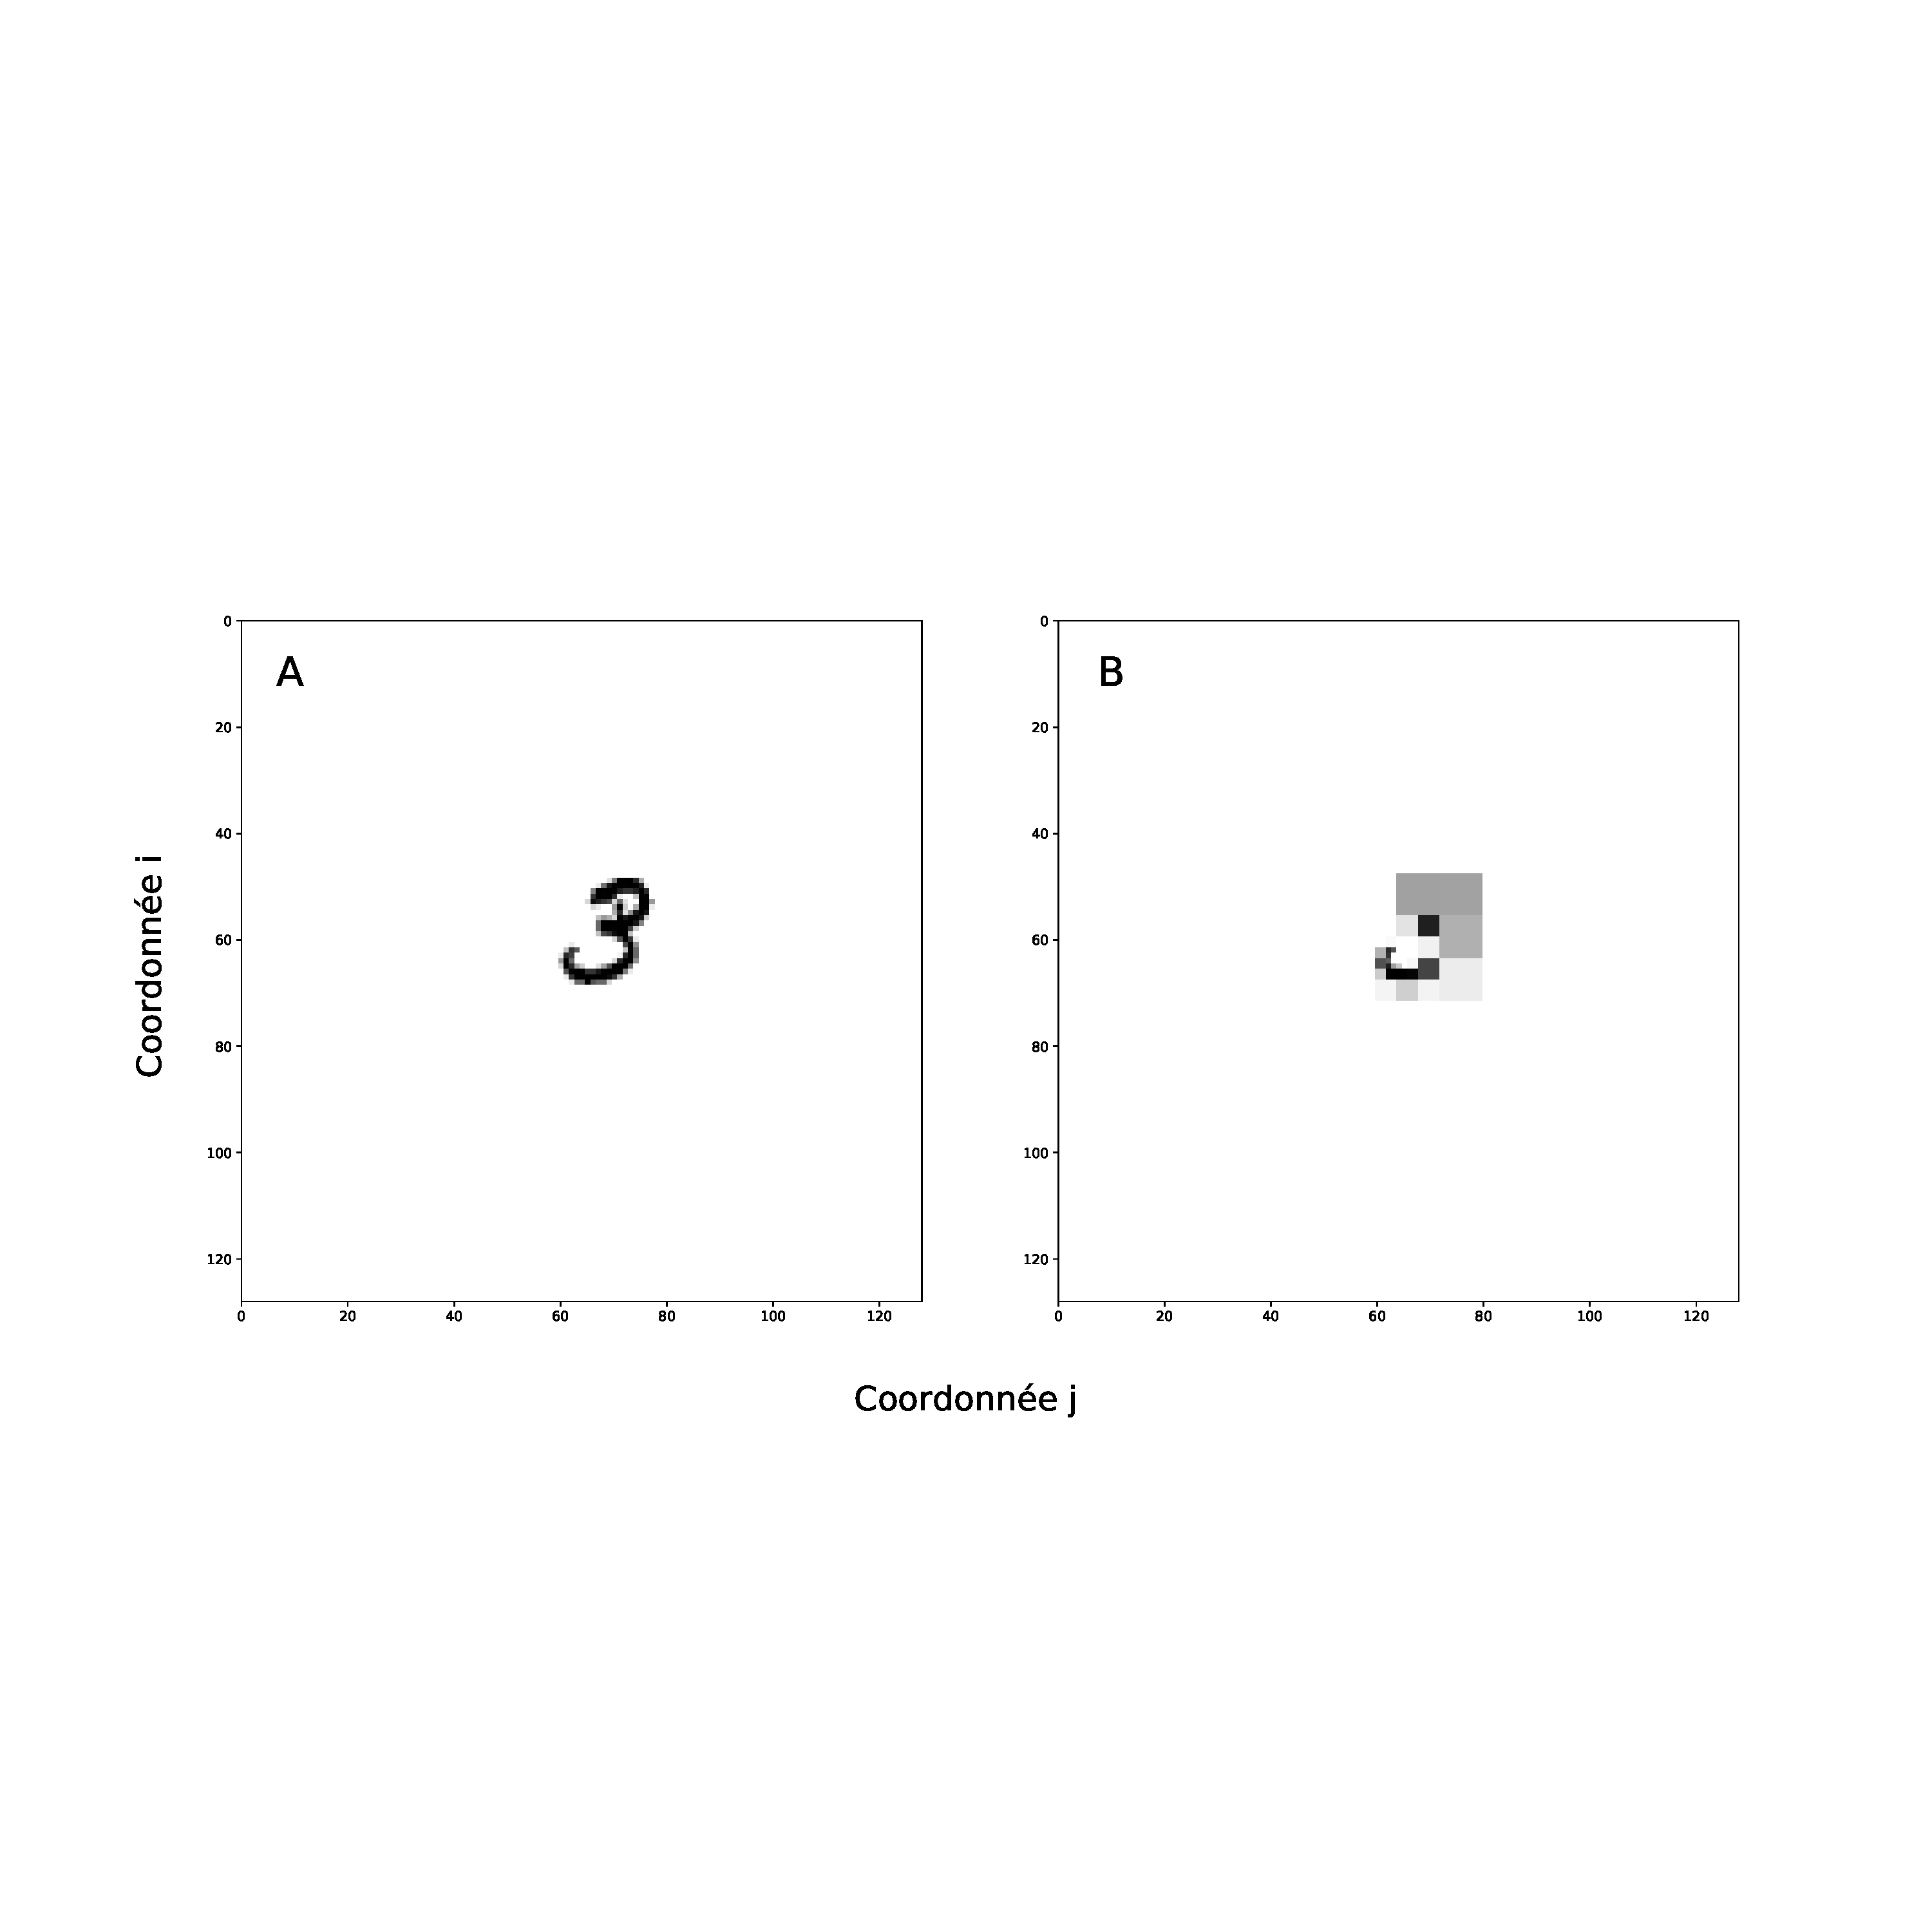
\includegraphics[scale=0.25]{Figures/wavelet_effect}
\decoRule %puts an aesthetic horizontal line below the image
\caption[Figure]{\textbf{A.} Image avant encodage pyramidal par ondelettes avec cible positionnée aux coordonnées $(i=-6,j=6)$ ; \textbf{B.} Image reconstruite d'après les valeurs des 70 coefficients d'ondelettes (taux de compression: $1-\frac{70}{128\times128}$)}
\label{fig:Wavelet_effect}
\end{figure}

\begin{figure}[th]
\centering
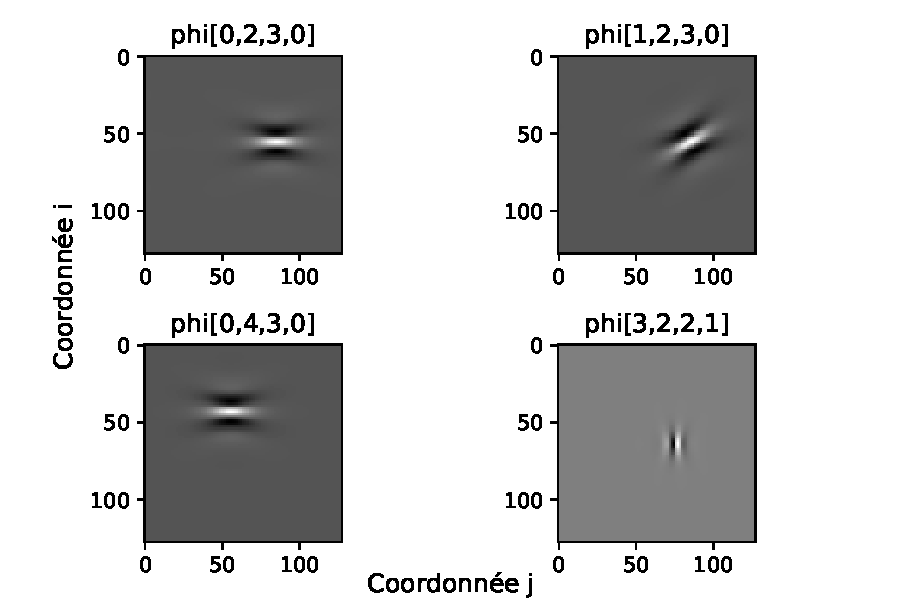
\includegraphics{Figures/Gabor_filter}
\decoRule %puts an aesthetic horizontal line below the image
\caption[Figure]{Exemples de filtres LogGabor tels qu'appliqués sur l'image originale, avec leurs paramètres respectifs (nombre total de filtre constituant \textit{LogPolar}: 400)}
\label{fig:Gabor_filter}
\end{figure}

\begin{figure}[th]
\centering
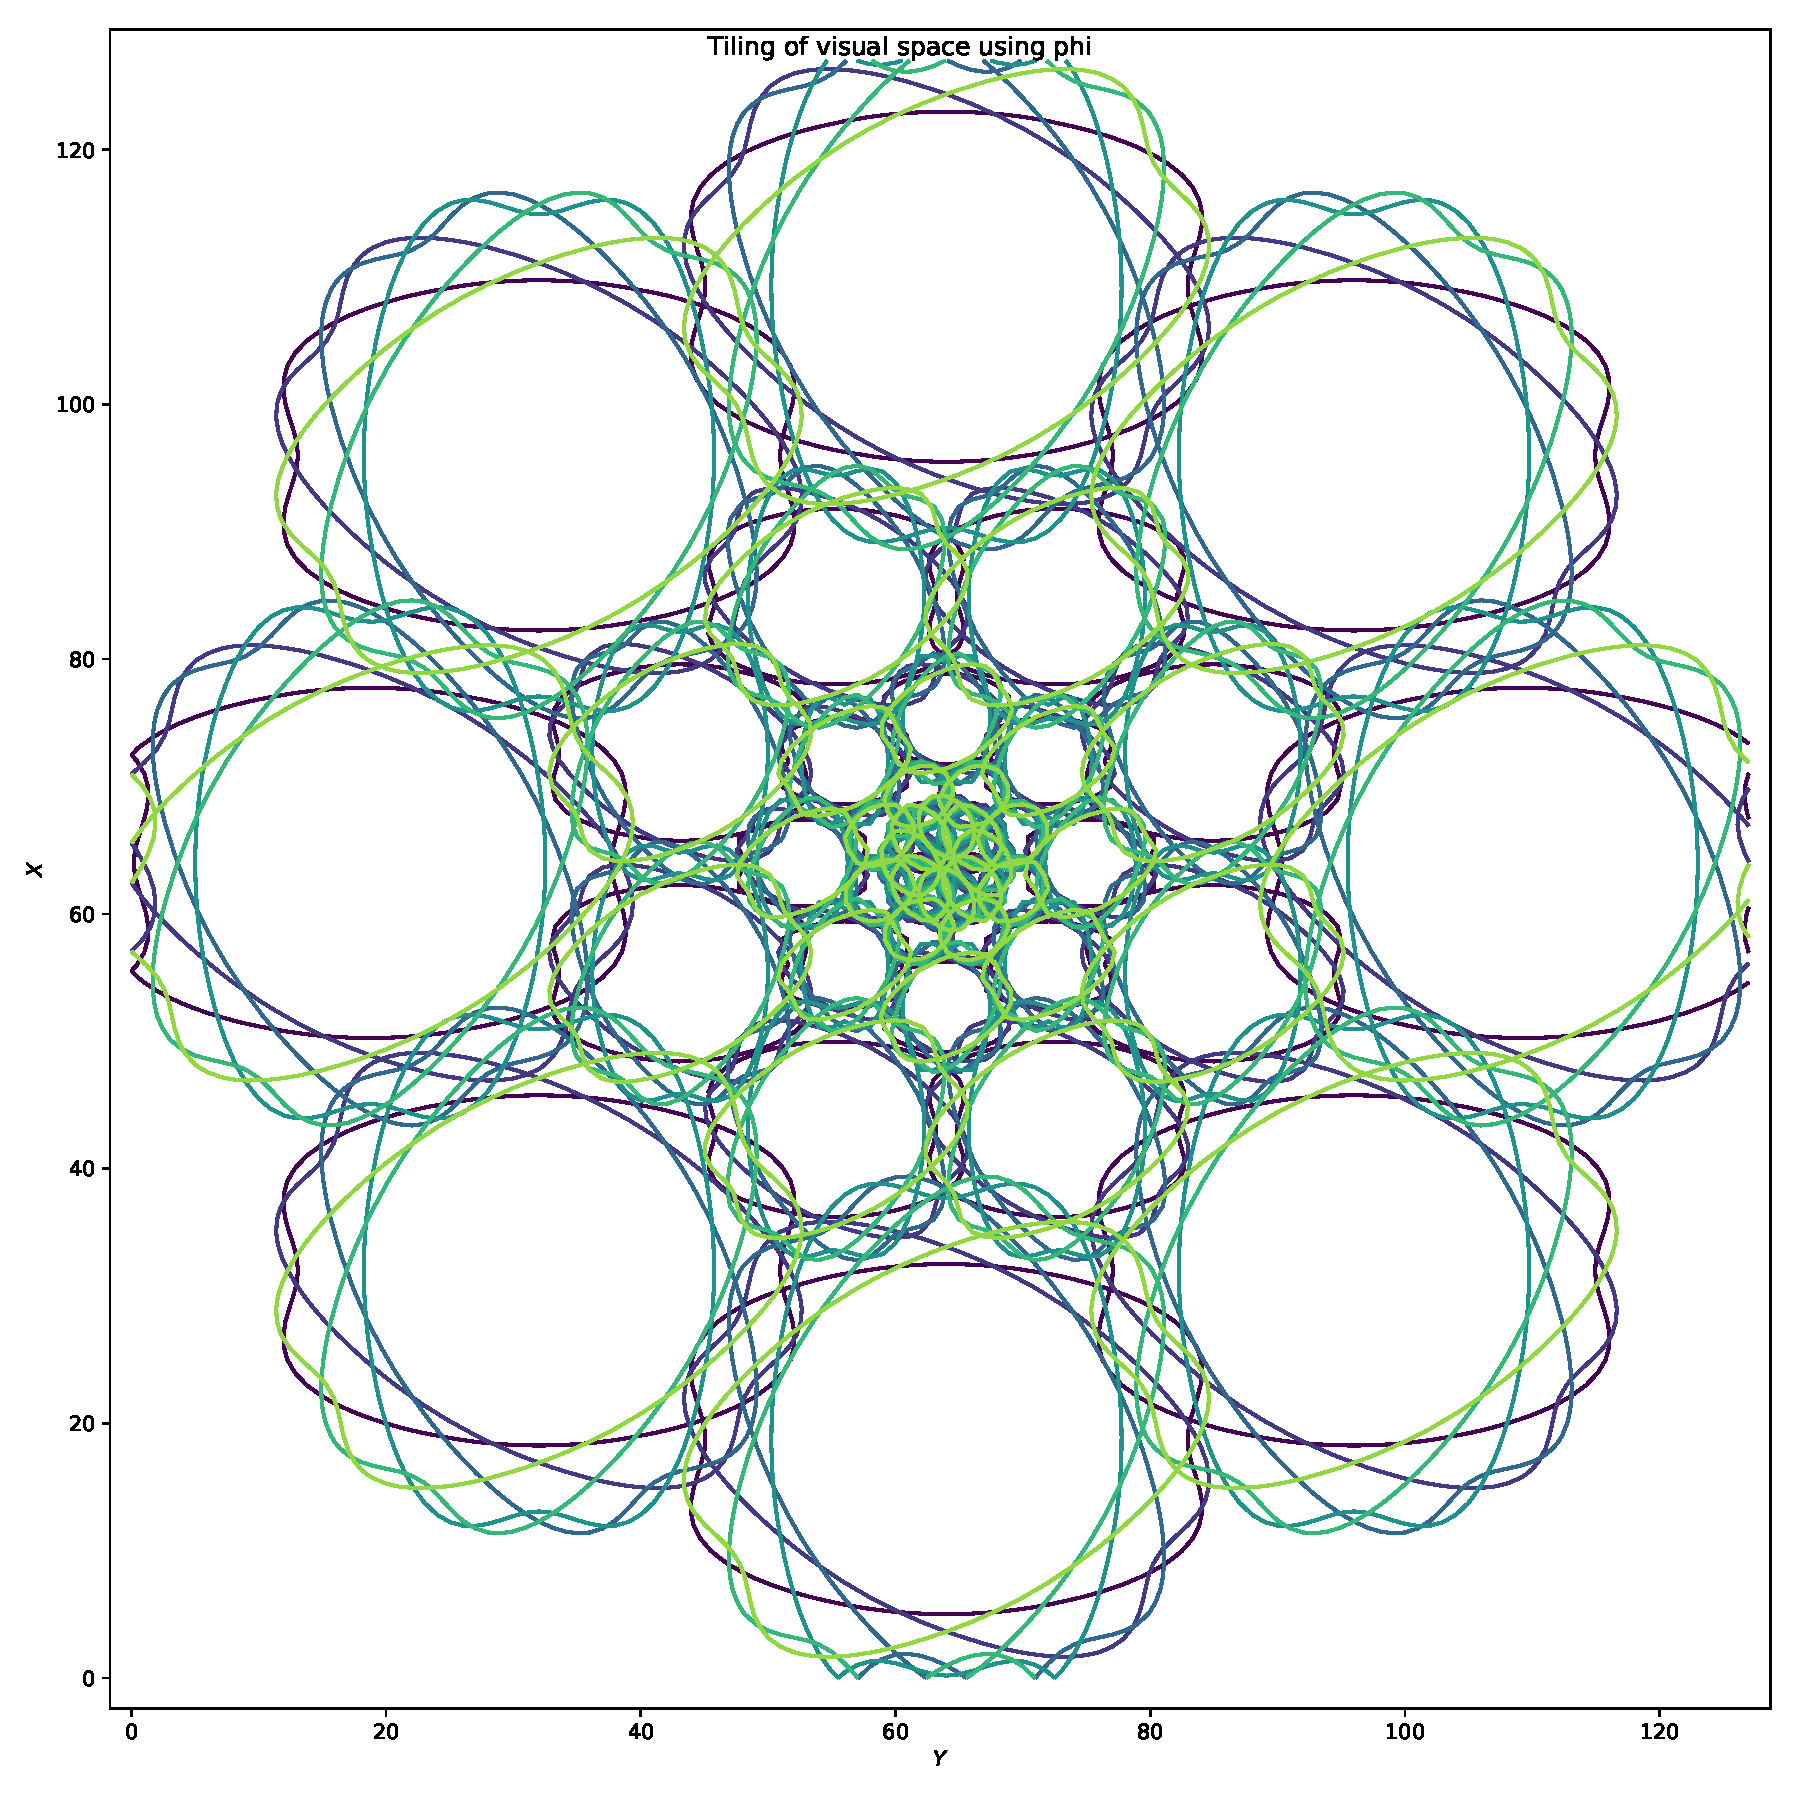
\includegraphics[scale=0.35]{Figures/LogPolar_shape}
\decoRule %puts an aesthetic horizontal line below the image
\caption[Figure]{Représentation graphique du filtre \textit{LogPolar} ($N_{theta}=6$,$N_{orient}=8$,$N_{scale}=5$,$N_{phase}=2$) }
\label{fig:LogPolar_shape}
\end{figure}

\begin{figure}[th]
\centering
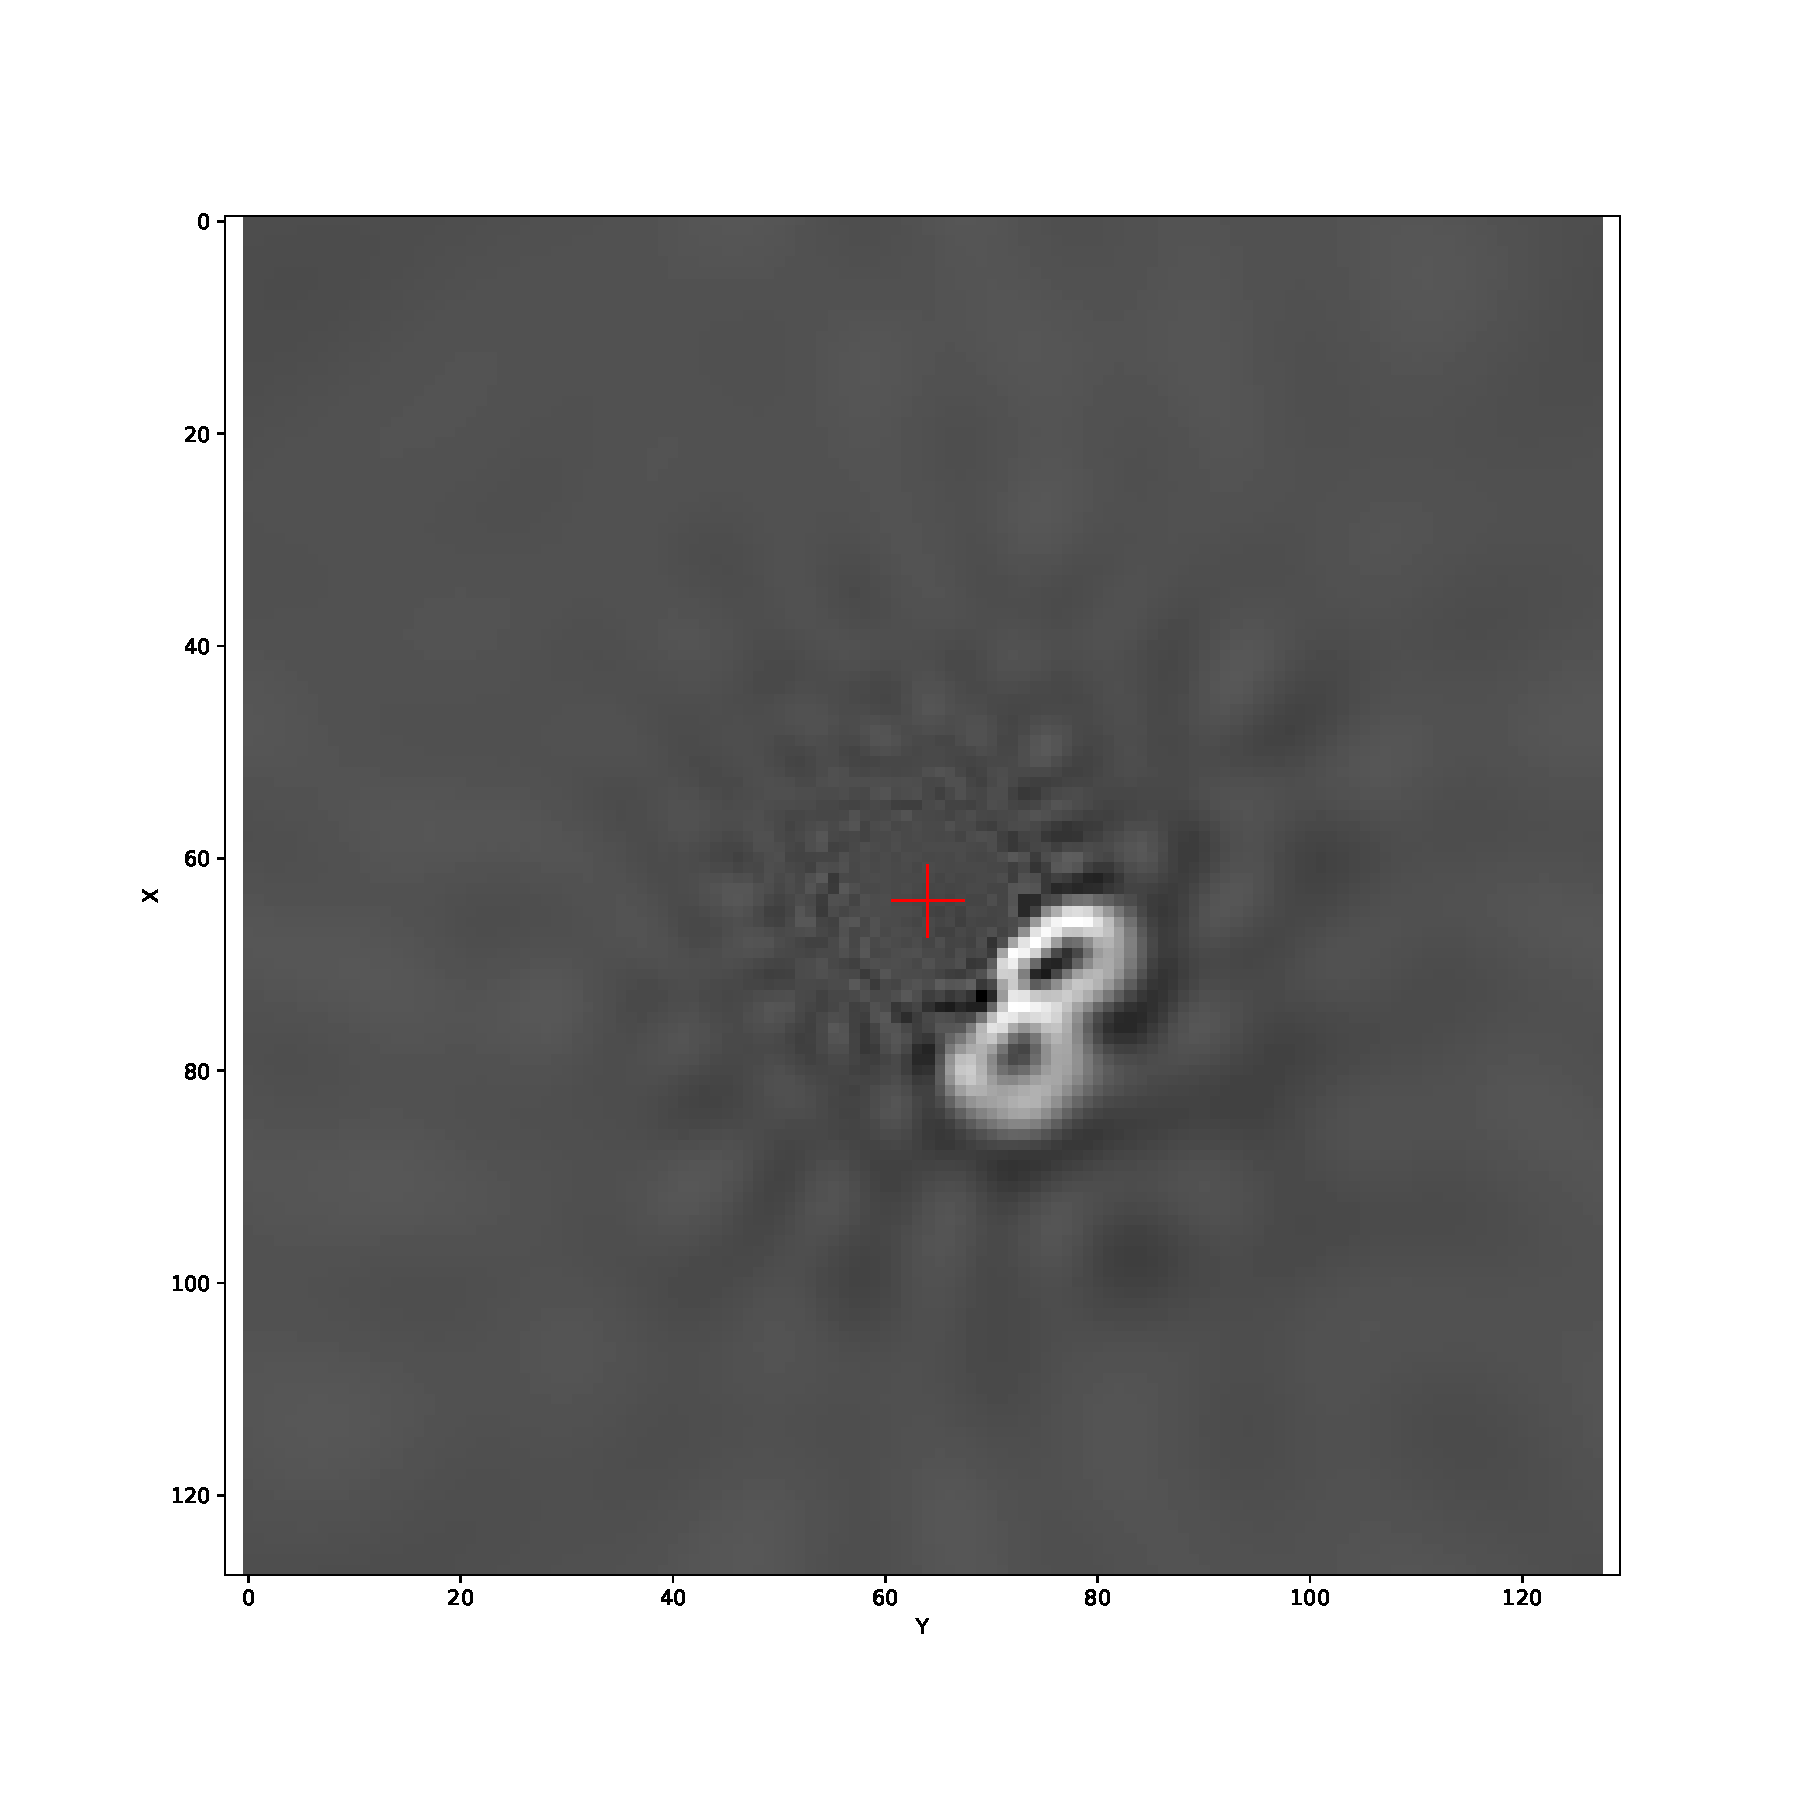
\includegraphics[scale=0.35]{Figures/LogPolar_effect}
\decoRule %puts an aesthetic horizontal line below the image
\caption[Figure]{Image reconstruite après transformation par le filtre \textit{LogPolar} ($N_{theta}=6$,$N_{orient}=8$,$N_{scale}=5$,$N_{phase}=2$) }
\label{fig:LogPolar_effect}
\end{figure}

\begin{algorithm}
\SetAlgoLined
$Image28 \leftarrow new\_MNIST\_example$\;
$(i,j) \leftarrow tirage\_aleatoire$\;
$Image128 \leftarrow creer\_Image128(Image28,(i,j))$\;
$x \leftarrow transformation(Image128(0,0))$\;
$\hat{i},\hat{j} \leftarrow (0,0)$\;
\While{$\|(i-\hat{i},j-\hat{j})\|>2$}{
  $\bigtriangleup i,\bigtriangleup j \leftarrow detecteur(x)$\;
  $\hat{i} \leftarrow \hat{i}+\bigtriangleup i$\;
  $\hat{j} \leftarrow \hat{j}+\bigtriangleup j$\;
  $x \leftarrow transformation(Image128,(\hat{i},\hat{j}))$\;
 }
\caption{Algorithme du modèle de reconnaissance visuelle\label{Algo}}
\end{algorithm}

%%%%% Résultats %%%%%

\begin{figure}[th]
\centering
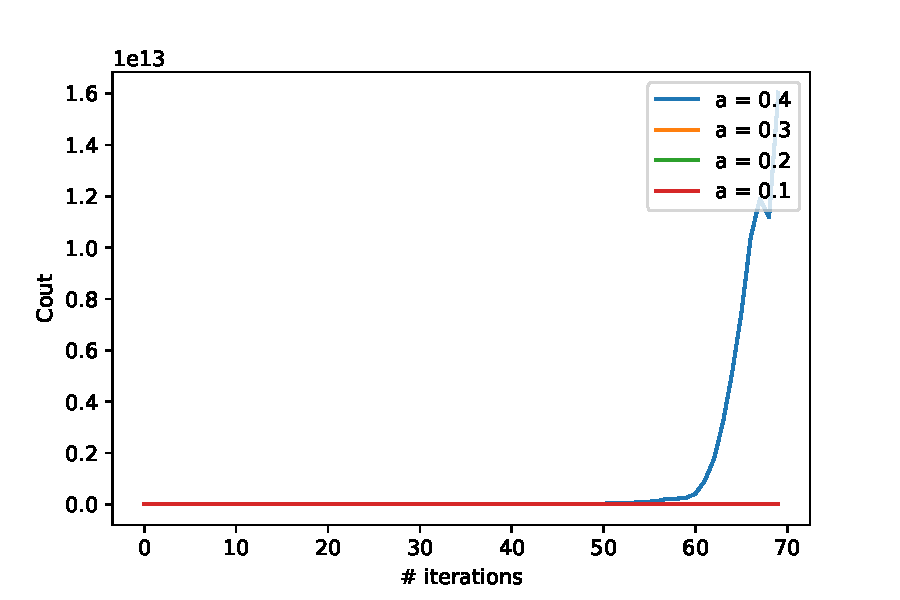
\includegraphics{Figures/Benchmarking_para_alpha_3}
\decoRule %puts an aesthetic horizontal line below the image
\caption[Figure]{Effet du paramètre alpha sur l'apprentissage dans le cadre d'un filtre \textit{Wavelets}}
\label{fig:benchmark_surApp2}
\end{figure}

\begin{figure}[th]
\centering
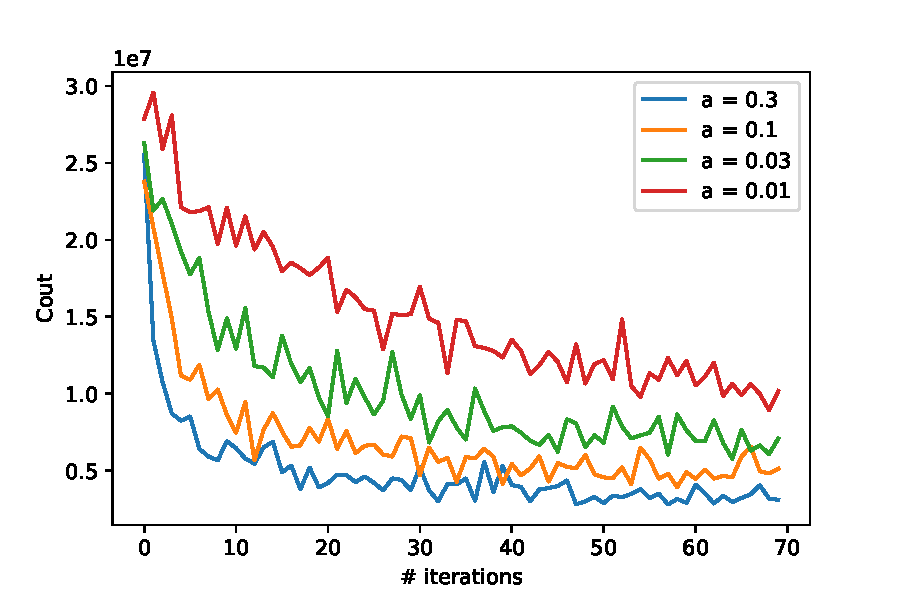
\includegraphics{Figures/Benchmarking_para_alpha}
\decoRule
\caption[Figure]{Effet du paramètre alpha sur l'apprentissage dans le cadre d'un filtre \textit{Wavelets}}
\label{fig:benchmark_alpha}
\end{figure}

\begin{figure}[th]
\centering
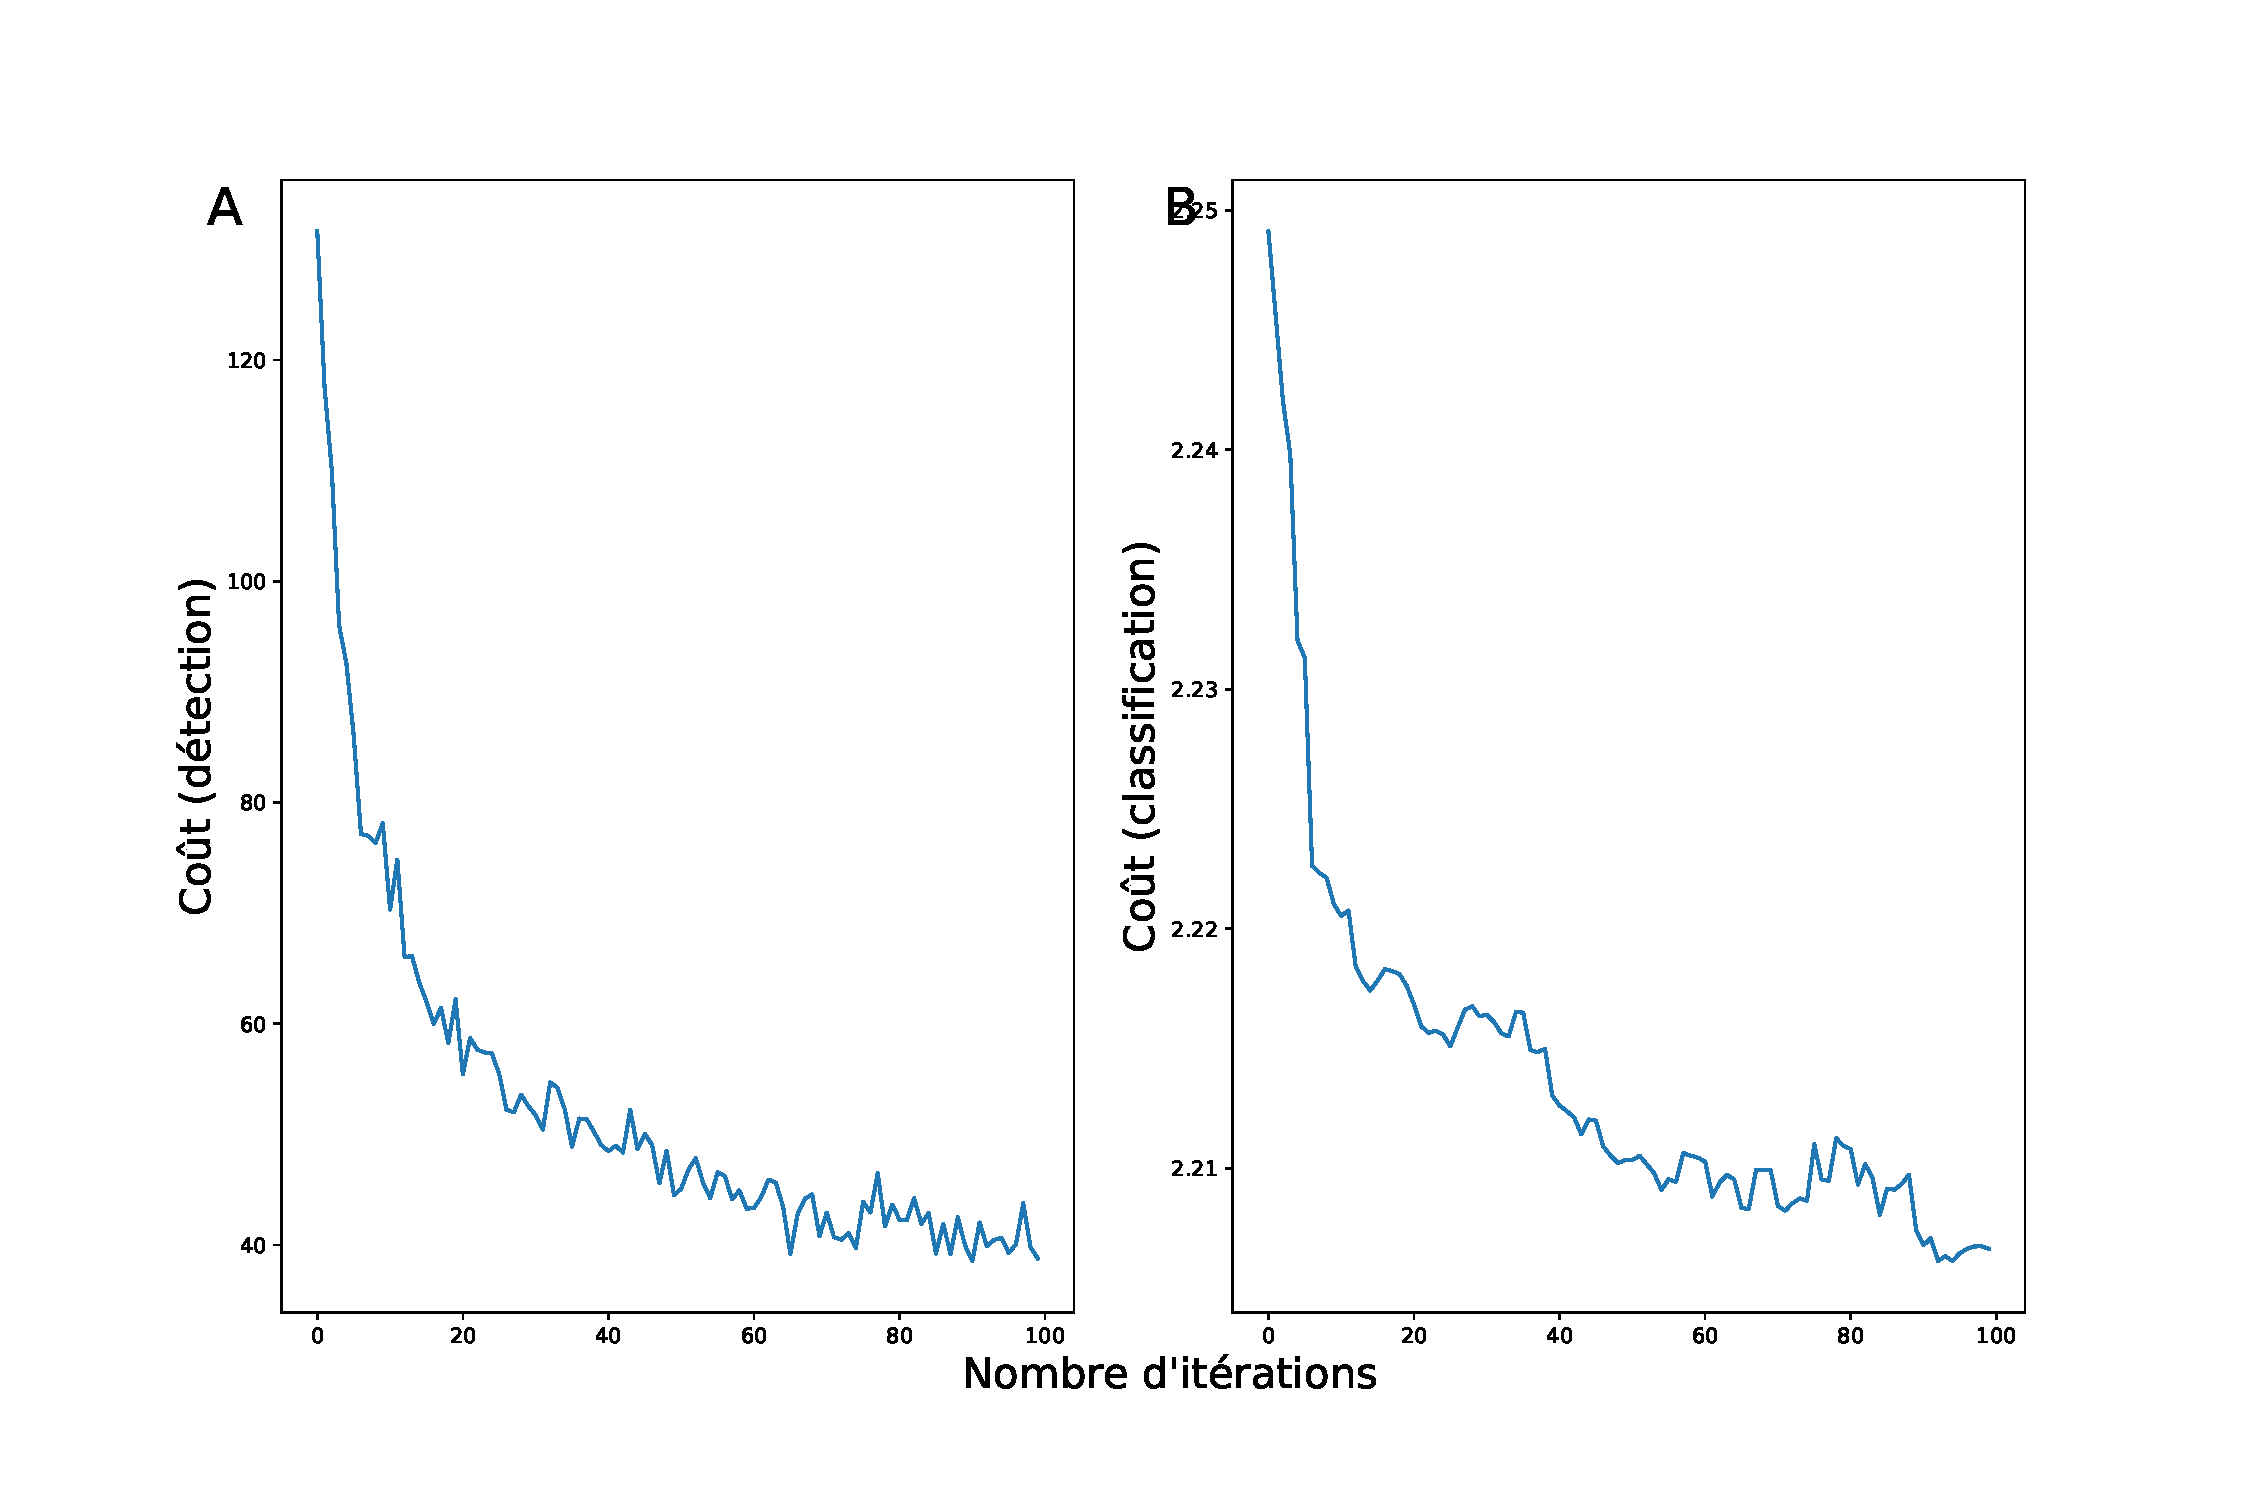
\includegraphics[scale=0.4]{Figures/logpolar_cost_learning}
\decoRule
\caption[Figure]{Quantification de la fonction de coût des couches \textit{détecteur} (gauche) et \textit{classifieur} (droite) lors de l'apprentissage, dans le cadre d'un filtre \textit{LogPolar} (taille de l'échantillon d'apprentissage :  10000, nombre d'itérations : 100, $\alpha_{detect}=0.0015$, $\alpha_{classif}=0.3$)}
\label{fig:logpolar_cost}
\end{figure}

\begin{figure}[th]
\centering
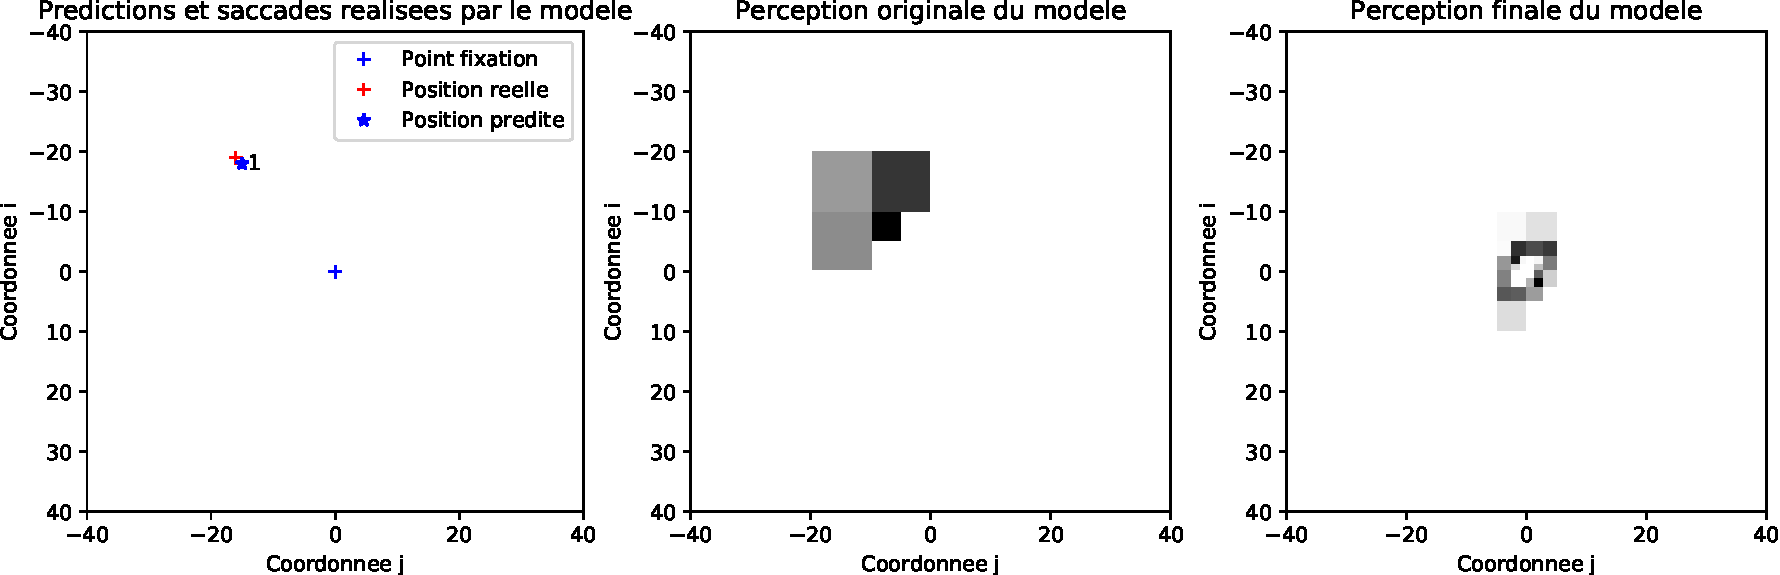
\includegraphics[scale=0.5]{Figures/saccades_wavelets}
\decoRule
\caption[Figure]{Exemple de perception et comportement saccadique du modèle entraîné, dans le cadre d'un filtre \textit{Wavelets}
\\ A gauche: Position de la fovéa avant et après saccade jusqu'à la position de la cible
\\ Au centre: Perception de l'agent avant saccade
\\ A droite: Perception de l'agent après saccade}
\label{fig:saccades_wavelets}
\end{figure}

\begin{figure}[th]
\centering
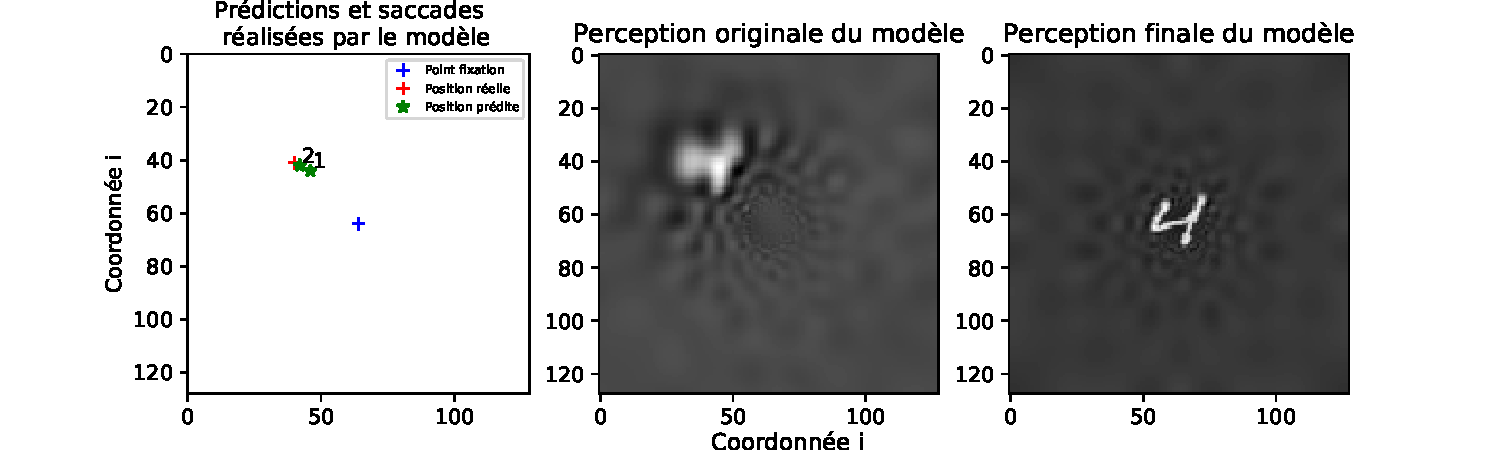
\includegraphics[scale=0.75]{Figures/saccades_logpolar}
\decoRule
\caption[Figure]{Exemple de perception et comportement saccadique du modèle entraîné, dans le cadre d'un filtre \textit{LogPolar}
\\ A gauche: Position de la fovéa avant et après saccades jusqu'à la position de la cible
\\ Au centre: Perception de l'agent avant saccades
\\ A droite: Perception de l'agent après saccades}
\label{fig:saccades_logpolar}
\end{figure}

\begin{figure}[th]
\centering
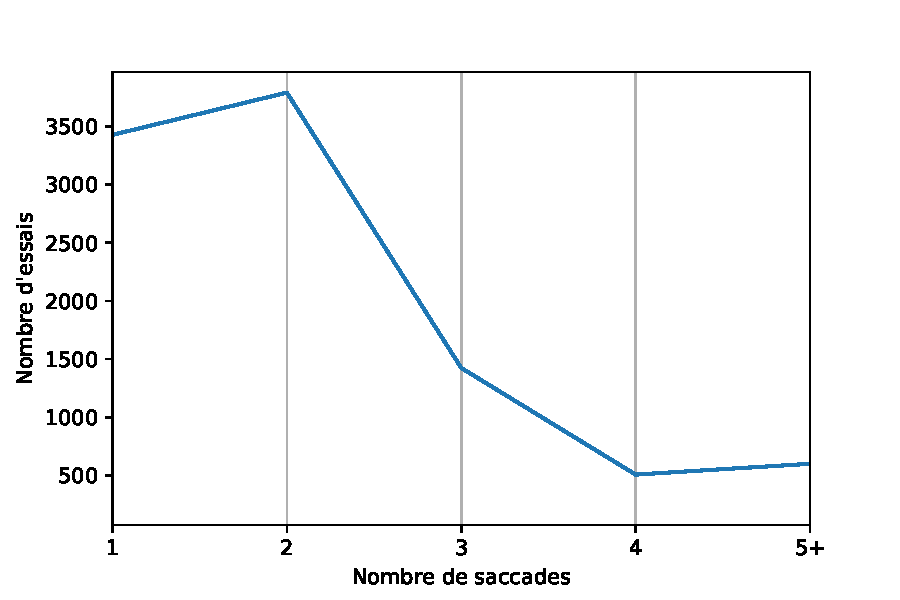
\includegraphics{Figures/logpolar_sacc_nombre}
\decoRule
\caption[Figure]{Nombre de saccades nécessaires pour atteindre la position de la cible au cours de 10000 essais, dans le cadre d'un filtre \textit{LogPolar} (taille de l'échantillon d'apprentissage :  10000, nombre d'itérations : 100, $\alpha_{detect}=0.0015$, $\alpha_{classif}=0.3$)}
\label{fig:sacc_nombre}
\end{figure}

\begin{figure}[th]
\centering
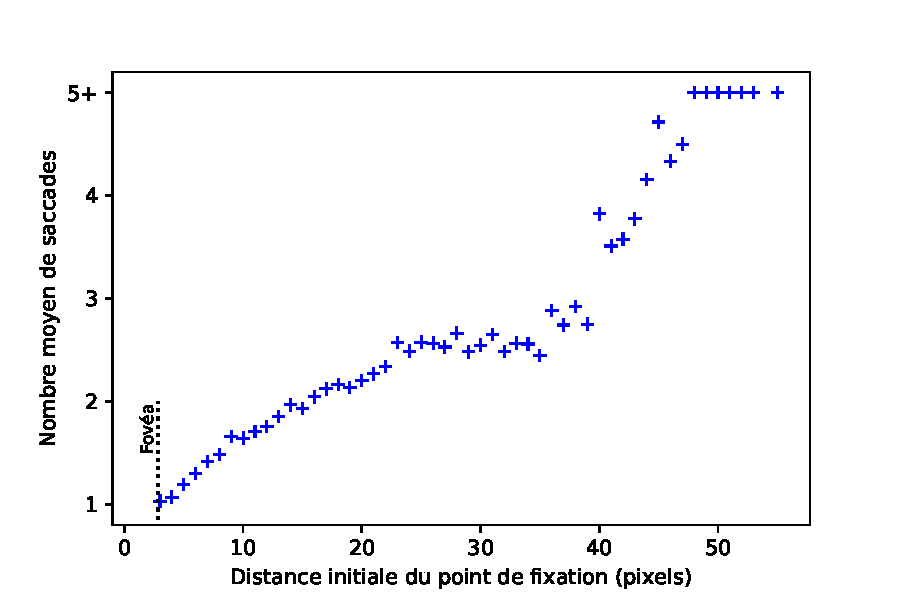
\includegraphics{Figures/logpolar_sacc_distance}
\decoRule
\caption[Figure]{Nombre moyen de saccades nécessaires pour atteindre la position de la cible en fonction de sa distance initiale du point de fixation au cours de 10000 essais, dans le cadre d'un filtre \textit{LogPolar} (taille de l'échantillon d'apprentissage :  10000, nombre d'itérations : 100, $\alpha_{detect}=0.0015$, $\alpha_{classif}=0.3$)}
\label{fig:sacc_distance}
\end{figure}

\begin{figure}[th]
\centering
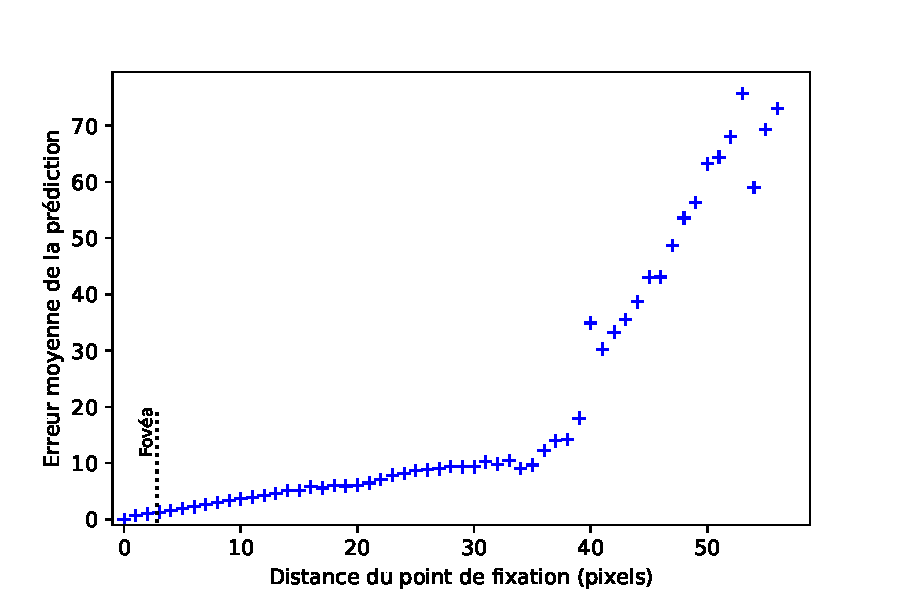
\includegraphics[scale=0.95]{Figures/logpolar_err_distance}
\decoRule
\caption[Figure]{Erreur moyenne lors de la prédiction de la position de la cible en fonction de sa distance du point de fixation au cours de 10000 essais, dans le cadre d'un filtre \textit{LogPolar} (taille de l'échantillon d'apprentissage :  10000, nombre d'itérations : 100, $\alpha_{detect}=0.0015$, $\alpha_{classif}=0.3$)}
\label{fig:err_distance}
\end{figure}